This project was based on a previous master thesis 'The Effect of Whole Barley Bread on the Risk of Cardiovascular Disease'\cite{Popovici2016}. Urine samples were collected in the previous research. The relevant contents of previous study\cite{Popovici2016} were summarized as the Background in this report.

\subsection{Research Questions and Study Design}
A double–blind randomized cross–over intervention was conducted. The research aimed at investigating the correlation between whole grain barley bread intake and \acrfull{cvd} risk factors. 

Figure \ref{fig:studes} (adapted from \cite{Popovici2016}) shows the schema of study design. Each intervention period lasted three weeks and was separated by a 2–week wash–out period.
During intervention period, the subjects consumed 2 custom-made rolls of \acrfull{wbb} or \acrfull{wwb} per day while maintaining a habitual diet.
14 healthy volunteer (6 men and 8 women) participated.

\begin{figure}[h]
    \centering
    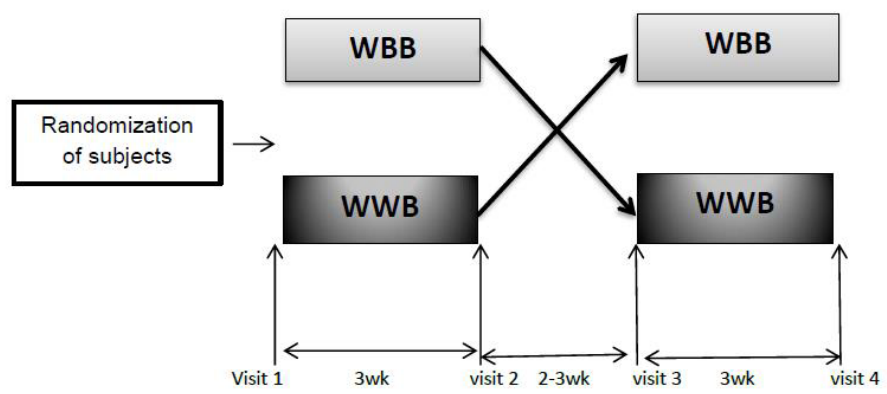
\includegraphics[scale=0.5]{studes}
    \caption{Schema of Study Design}
        \label{fig:studes}
\end{figure}

\subsection{\acrshort{cvd} Risk Factors and Other Health Status Indicators}
\acrfull{tc}, \acrfull{ldlc}, \acrfull{hdlc}, \acrfull{tg}, \acrfull{crp}, fasting glucose and fasting insulin were measured both before and after intervention. 

Besides \acrshort{cvd} risk factors, body weight and waist circumference were also measured. Urine and blood samples for this research were also collected during each visit. 

\subsection{Conclusions}
No significant effect of treatment was detected for \acrshort{tc} (p = 0.31), \acrlong{tg} (p = 0.11), CRP (p = 0.62), fasting insulin and glucose (p= 0.78 and 0.51, respectively), HDL–C and LDL–C (p = 0.32 and 0.25, respectively). 
This could be attributed to small sample size and short intervention period. In addition, the storage and food processing of bread could also affect the results\cite{Popovici2016}.